\begin{center}

\includegraphics[width=0.3\textwidth]{content/3/chapter6/images/24.png}\\
Cippi在扎辫子
\end{center}

std::jthread代表连接线程。除了C++11中的\href{https://en.cppreference.com/w/cpp/thread/thread}{std::thread}之外,std::jthread会在析构函数中自动汇入,并且可以协作中断。

下表简要概述了std::jthread t功能。更多详情请参考\href{https://en.cppreference.com/w/cpp/thread/jthread}{cppreference.com}。

\begin{table}[H]
\centering
\begin{tabular}{ll}
\textbf{函数}                                                             & \textbf{std::jthread t的函数描述}                                        \\ \hline
t.join()                                                                    & 等待线程t完成执行。            \\  \hline
t.detach()                                                                  & 独立执行创建的线程t。 \\ \hline
t.joinable()                                                                & 若线程t仍然是可汇入的,则返回true。                 \\ \hline
\begin{tabular}[c]{@{}l@{}}t.get\_id() and \\ std::this\_thread::get\_id()\end{tabular} &
返回线程的id。 \\ \hline
std::jthread::hardware\_concurrency()                                       & 表示可以并发运行的线程数。  \\ \hline
std::this\_thread::sleep\_until(absTime)                                    & 线程t进入睡眠状态,直到时间点absTime。           \\ \hline
std::this\_thread::sleep\_for(relTime)                                      & 线程t进入睡眠状态,时间为relTime。           \\ \hline
std::this\_thread::yield()                                                  & 允许系统运行另一个线程。                   \\ \hline
\begin{tabular}[c]{@{}l@{}}t.swap(t2) and \\ std::swap(t1, t2)\end{tabular} & 交换线程。                                          \\ \hline
t.get\_stop\_source() &
\begin{tabular}[c]{@{}l@{}}返回与共享停止状态关联的std::stop\_source对象。\end{tabular} \\ \hline
t.get\_stop\_token() &
\begin{tabular}[c]{@{}l@{}}返回与共享停止状态关联的std::stop\_token对象。\end{tabular} \\ \hline
t.request\_stop()                                                           & 通过共享停止状态停止执行请求。          \\ \hline
\end{tabular}
\end{table}

\subsubsubsection{6.6.1\hspace{0.2cm}自动汇入}

这是std::thread的一种非直观行为。若std::thread仍然可汇入,\href{https://en.cppreference.com/w/cpp/error/terminate}{std::terminate}将在其析构函数中调用。若既没有调用thr.join(),也没有调用thr.detach(),那么线程thr是可汇入的。

\begin{lstlisting}[style=styleCXX]
// threadJoinable.cpp

#include <iostream>
#include <thread>

int main() {
	std::cout << '\n';
	std::cout << std::boolalpha;
	
	std::thread thr{[]{ std::cout << "Joinable std::thread" << '\n'; }};
	
	std::cout << "thr.joinable(): " << thr.joinable() << '\n';
	
	std::cout << '\n';
	
}
\end{lstlisting}

执行时,程序终止。

\begin{center}
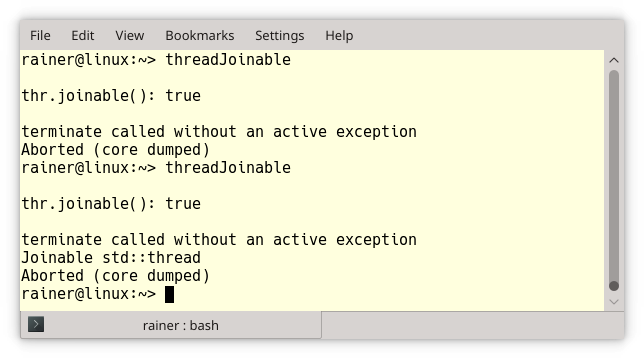
\includegraphics[width=0.7\textwidth]{content/3/chapter6/images/25.png}\\
\end{center}

std::thread的两次执行都终止。在第二次运行中,线程thr有足够的时间显示它的消息:" Joinable std::thread "。

下一个例子中,使用来自C++20标准的std::jthread。

\begin{lstlisting}[style=styleCXX]
// jthreadJoinable.cpp

#include <iostream>
#include <thread>

int main() {
	std::cout << '\n';
	std::cout << std::boolalpha;
	
	std::jthread thr{[]{ std::cout << "Joinable std::thread" << '\n'; }};
	
	std::cout << "thr.joinable(): " << thr.joinable() << '\n';
	
	std::cout << '\n';
}
\end{lstlisting}

现在,若线程thr是可汇入的,则会在析构函数中使用自动汇入。

\begin{center}
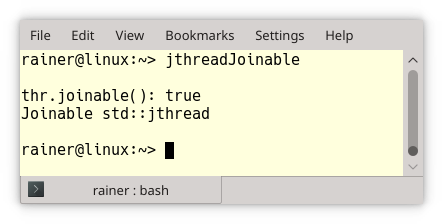
\includegraphics[width=0.6\textwidth]{content/3/chapter6/images/26.png}\\
\end{center}

\subsubsubsection{6.6.2\hspace{0.2cm}std::jthread的协作中断}

举一个简单的例子来了解大体的情况。

\begin{lstlisting}[style=styleCXX]
// interruptJthread.cpp

#include <chrono>
#include <iostream>
#include <thread>

using namespace::std::literals;

int main() {

	std::cout << '\n';
	
	std::jthread nonInterruptible([]{
		int counter{0};
		while (counter < 10){
			std::this_thread::sleep_for(0.2s);
			std::cerr << "nonInterruptible: " << counter << '\n';
			++counter;
		}
	});
	
	std::jthread interruptible([](std::stop_token stoken){
		int counter{0};
		while (counter < 10){
			std::this_thread::sleep_for(0.2s);
			if (stoken.stop_requested()) return;
			std::cerr << "interruptible: " << counter << '\n';
			++counter;
		}
	});
	
	std::this_thread::sleep_for(1s);
	
	std::cerr << '\n';
	std::cerr << "Main thread interrupts both jthreads" << '\n';
	nonInterruptible.request_stop();
	interruptible.request_stop();
	
	std::cout << '\n';

}
\end{lstlisting}

主程序中,我启动了nonInterruptible和interruptible两个线程(第13行和第22行)。与不可中断线程不同,可中断线程获得std::stop\_token,并在第26行中使用它来检查是否中断:stoken.stop\_requested()。停止请求的情况下,Lambda函数返回,因此线程结束,调用interruptible.request\_stop()(第37行)停止请求。但这并不适用于之前的调用nonInterruptible.request\_stop(),所以调用无效。

\begin{center}
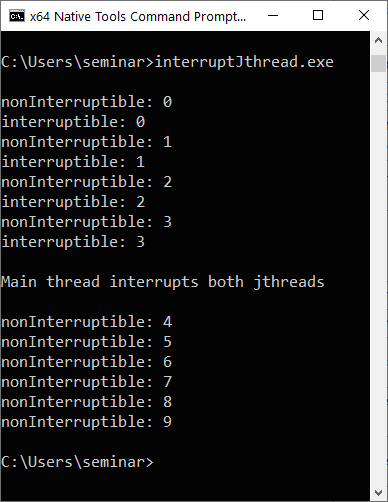
\includegraphics[width=0.5\textwidth]{content/3/chapter6/images/27.png}\\
\end{center}

\newpage

























